\documentclass[sigconf,nonacm,screen]{acmart}
\usepackage{filecontents}
\usepackage{textcomp}
\usepackage{pgfplots}
\usetikzlibrary{patterns}
\usepackage{ifthen}
\usepgfplotslibrary{groupplots}
\RequirePackage{keyval}
\usepackage{multirow}
\usepackage{multicol}
\usepackage{csvsimple}
\usepackage[utf8]{inputenc}
\newcounter{row}
\newcounter{col}
\usepackage{wrapfig}
\usepackage{textgreek}
\usepackage[inline]{enumitem}
% \usepackage[table]{xcolor}
\usetikzlibrary{matrix, positioning}
\usetikzlibrary{patterns,tikzmark}
\usetikzlibrary{matrix,decorations.pathreplacing,calc}
\usepackage{hf-tikz}
\usepackage{pifont}
\usepackage{subfig}
\usetikzlibrary{chains,fit,shapes}
\usetikzlibrary{arrows.meta,
    chains,
    positioning,
    shapes.symbols}
\usetikzlibrary{decorations,calligraphy}
\usepackage{pgfplotstable}
\usepgfplotslibrary{statistics}
%\pgfplotsset{compat=newest}
\usetikzlibrary{matrix,calc}
\usetikzlibrary{fit}
\usepackage{xfp}
\usepackage{mathtools}

\usetikzlibrary{positioning}

\usepackage{makecell}
%\usepackage{tabu}
\usepackage{tikz}
\usetikzlibrary{trees}

%\pgfplotsset{compat=1.8}
\pgfplotsset{compat=1.12}


\usepgfplotslibrary{fillbetween}

\usepackage{filecontents}
% \usetikzlibrary{pgfplots.groupplots}
% \pgfplotsset{compat=1.9}

% \usepackage[utf8]{inputenc}
% \usepackage[ngerman]{babel}
% \usepackage{pgfplots}
% \pgfplotsset{compat=1.9}
% \usetikzlibrary{
%   pgfplots.groupplots,
%   matrix
% }
% \usepackage{siunitx}

\newtheorem{theorem}{Theorem}
\newtheorem{definition}{Definition}
\newcommand{\eat}[1]{}

\definecolor{bluegreen}{RGB}{3, 166, 155}
\definecolor{pitchblack}{RGB}{0, 0, 0}
\definecolor{lightbeige}{RGB}{255, 251, 241}
\definecolor{mediumgray}{RGB}{183, 183, 183}
\definecolor{mygreen}{rgb}{0,0.6,0}
\definecolor{mygray}{rgb}{0.5,0.5,0.5}
\definecolor{mymauve}{rgb}{0.58,0,0.82}
\definecolor{keywords}{RGB}{255,0,90}
\definecolor{comments}{RGB}{0,0,113}
\definecolor{red}{RGB}{255,0,0}
\definecolor{green}{RGB}{0,255,0}
\definecolor{navy}{RGB}{0,0,128}
\definecolor{DarkGrenen}{RGB}{0,100,0}
\definecolor{DarkOliveGreen}{RGB}{85,107,47}
\definecolor{saddlebrown}{RGB}{139,69,19}
\definecolor{gold}{RGB}{252,194,1}
\definecolor{tug}{RGB}{247,1,70}
\definecolor{tugb}{RGB}{120,137,251}

\definecolor{color01}{RGB}{159,96,0}
\definecolor{color02}{RGB}{43,85,128}


\definecolor{blue0}{RGB}{153,153,153}
\definecolor{blue1}{RGB}{77,77,77}%
\definecolor{blue2}{RGB}{165,71,209}
\definecolor{blue3}{RGB}{77,10,142}
\definecolor{blue4}{RGB}{74,139,203}
\definecolor{blue5}{RGB}{40,40,190}

\definecolor{color1}{RGB}{100,149,237} % corn flower blue
\definecolor{color2}{RGB}{153,153,153} % light gray
\definecolor{color3}{RGB}{0,0,0} % black
\definecolor{color4}{RGB}{255,165,0} % orange
\definecolor{color5}{RGB}{255,69,0} % orange red
\definecolor{color6}{RGB}{77,77,77} % dark gray
\definecolor{color7}{RGB}{31,119,180}
\definecolor{color8}{RGB}{7,77,125}
\definecolor{color9}{RGB}{153,216,201}


\definecolor{teal1}{RGB}{31, 111, 111}
\definecolor{teal2}{RGB}{84, 161, 161}
\definecolor{teal3}{RGB}{159, 200, 200}

\definecolor{dred1}{RGB}{160, 0, 0}
\definecolor{dred2}{RGB}{196, 102, 102}
\definecolor{dred3}{RGB}{216, 166, 166}


\definecolor{dblue1}{RGB}{32, 102, 168}
\definecolor{dblue2}{RGB}{53, 148, 204}
\definecolor{dblue3}{RGB}{140, 197, 227}

\definecolor{totalcolor}{RGB}{2, 152, 215}
\definecolor{mvcolor}{RGB}{248, 163, 47}
\definecolor{dvcolor}{RGB}{203, 70, 39}



% Enable this two commands when you want to extract diagrams in extra files, then run "make"
\usetikzlibrary{external}
\tikzexternalize[prefix=plots/] %  activate

\usetikzlibrary{positioning}

\sloppy
\clubpenalty = 10000
\widowpenalty = 10000
\brokenpenalty = 10000
\frenchspacing


\makeatletter
\def\pgfplots@drawaxis@lines@preparediscont@for#1{%
        \ifnum\csname pgfplots@#1axisdiscontnum\endcsname>0
                \begingroup
                % this group employs several temporary dimension registers
                % and is therefor scoped:
                \let\disstart=\pgf@ya
                \let\disend=\pgf@yb
                \disend=\csname pgfplots@#1max@reg\endcsname
                \advance\disend by -\csname pgfplots@#1min@reg\endcsname
                \disend=\csname pgfplots@#1@veclength\endcsname\disend
                \ifcase\csname pgfplots@#1axisdiscontnum\endcsname\relax
                        % has already been checked above.
                \or
                        \def\discontstyle{decoration={zigzag,segment length=5pt, amplitude=2pt}}%
                        \advance \disend by -8pt
                \or
                        \def\discontstyle{decoration={ticks,segment length=4pt, amplitude=8pt}}%
                        \advance \disend by -4pt
                \fi
                \pgfplotscoordmath{#1}{datascaletrafo get params}%
                % if #1max + shift < 0pt  (shift is 0 without the scaling trafo)
                \ifdim\csname pgfplots@#1max@reg\endcsname<-\pgfplotsretvalb pt
                        % swap start and end
                        \disstart=\disend
                        \disend=2pt
                \else
                        \disstart=2pt
                \fi
                % carry local computations outside of group:
                \xdef\pgfplots@glob@TMPa{%
                        \noexpand\def\expandafter\noexpand\csname #1disstart\endcsname{\the\disstart}%
                        \noexpand\def\expandafter\noexpand\csname #1disend\endcsname{\the\disend}%
                        \noexpand\pgfkeysdef{/tikz/#1discont}{\noexpand\pgfkeysalso{\discontstyle}}%
                }%
                \endgroup
                \pgfplots@glob@TMPa
        \else
                \expandafter\def\csname #1disstart\endcsname{0pt}%
                \expandafter\def\csname #1disend\endcsname{0pt}%
                \pgfkeyslet{/tikz/#1discont}=\pgfutil@empty
        \fi
}%
\makeatother



\begin{document}
\title[Query Processing by Data Catalog]{Query Processing by Data Catalog}

\author{Saeed Fathollahzadeh} 
\orcid{0000-0003-3723-6191}
\affiliation{
\institution{Concordia University}
\country{Canada}}

\renewcommand{\shortauthors}{Saeed Fathollahzadeh}

\maketitle

%    \tikzsetnextfilename{Experiment1-Data-Profiling}
%     \begin{figure*}[h]
%         \centering
%         \newcommand{\addplotDataProfilling}[1]{
	   \addplot[xshift=0, draw=black,line width=0.15pt, fill=tugb] 
	   table[y=time, col sep=comma, x=dataset] {../archive/Final-Results/Experiment1_Data_Profile.dat};
     %\label{leg_dataprofile} 
};

\begin{tikzpicture}[
  every axis/.style={
    major x tick style = {draw=none},
    % ybar stacked,
    ymode=log,
    xtick style={draw=none},		
    every major tick/.append style={ thick,major tick length=2.5pt, gray},
    axis line style={gray},
    ybar,        
    ymin=20000,
    ymax=600000,
    log ticks with fixed point,
    y tick label style={/pgf/number format/1000 sep={}},
    x tick label style={/pgf/number format/1000 sep={}},
    scaled y ticks=false,
    enlarge y limits={0.02,upper},
    enlarge x limits=0.02,
    ylabel={Execution Time[s]},
    ytick={20000,40000,80000,160000,320000,600000},
    yticklabels={0, 40, 80, 160, 320,600},
    ytick align=outside,
    xtick pos=left,
    ytick pos=left,
    yticklabel style = {font=\scriptsize},
    ylabel style = {font=\scriptsize, yshift=-1pt, xshift=-5pt},
    xticklabel style = {font=\scriptsize, xshift=0pt,yshift=2pt ,rotate=90},
    height=0.35\columnwidth,
    width=1.4\columnwidth,    
    bar width=8pt,
    ymajorgrids=true,
    grid style=dotted,   
    minor grid style={gray!50}, 
    xtick = data,
    symbolic x coords={Higgs,Albert,Click-Prediction,Census,Heart-Statlog,KDDCup99,Road-Safety,Drug-Directory,Okcupid-Stem,Walking-Activity,PASS,Aloi,MD-MIX-Mini,Dionis,Meta-Album-BRD,Balance-Scale,Breast-w,CMC,Credit-g,Diabetes,Tic-Tac-Toe,Eucalyptus,PC1,Airlines,Jungle-Chess}, 
    legend image code/.code={\draw [#1] (0cm,-0.1cm) rectangle (0.3cm,0.2cm); },
  }	 
]
	
\begin{axis}%[hide axis]
  \addplotDataProfilling{-16pt};	  	  
\end{axis}
\end{tikzpicture}

%         \caption{Runtime}
%     \end{figure*} 

    % \tikzsetnextfilename{Experiment1-Breast-w}
    % \begin{figure*}[h]
    %     \centering
    %     \input{exp1_catalog/Experiment1-Breast-w.tex}
    %     \caption{Experiment1-Breast-w}
    % \end{figure*} 

    % \tikzsetnextfilename{Experiment1-Credit-g}
    % \begin{figure*}[h]
    %     \centering
    %     \input{exp1_catalog/Experiment1-Credit-g}
    %     \caption{Experiment1-Credit-g}
    % \end{figure*} 

    % \tikzsetnextfilename{Experiment1-Diabetes}
    % \begin{figure*}[h]
    %     \centering
    %     \input{exp1_catalog/Experiment1-Diabetes}
    %     \caption{Experiment1-Diabetes}
    % \end{figure*} 

    % \tikzsetnextfilename{Experiment1-Tic-Tac-Toe}
    % \begin{figure*}[h]
    %     \centering
    %     \input{exp1_catalog/Experiment1-Tic-Tac-Toe}
    %     \caption{Experiment1-Tic-Tac-Toe}
    % \end{figure*} 

    % \tikzsetnextfilename{Experiment1-PC1}
    % \begin{figure*}[h]
    %     \centering
    %     \input{exp1_catalog/Experiment1-PC1}
    %     \caption{Experiment1-PC1}
    % \end{figure*} 

    % \tikzsetnextfilename{Experiment1-Airlines}
    % \begin{figure*}[h]
    %     \centering
    %     \input{exp1_catalog/Experiment1-Airlines}
    %     \caption{Experiment1-Airlines}
    % \end{figure*}

    %  \tikzsetnextfilename{Experiment1-Balance-Scale}
    % \begin{figure*}[h]
    %     \centering
    %     \input{exp1_catalog/Experiment1-Balance-Scale}
    %     \caption{Experiment1-Balance-Scale}
    % \end{figure*}

    % \tikzsetnextfilename{Experiment1-CMC}
    % \begin{figure*}[h]
    %     \centering
    %     \input{exp1_catalog/Experiment1-CMC}
    %     \caption{Experiment1-CMC}
    % \end{figure*}

    % \tikzsetnextfilename{Experiment1-Eucalyptus}
    % \begin{figure*}[h]
    %     \centering
    %     \input{exp1_catalog/Experiment1-Eucalyptus}
    %     \caption{Experiment1-Eucalyptus}
    % \end{figure*}

    \tikzsetnextfilename{Experiment1-Jungle-Chess}
    \begin{figure*}[h]
        \centering
        \newcommand{\addCatDBPerformance}[7]{
  \nextgroupplot[ymin=0,ymax=1,
      ytick={0,0.2,0.4,0.6,0.8,1.0},
      yticklabels={#3},
      height=0.35\columnwidth,
      width=.27\columnwidth,
      bar width=3pt,
      enlarge x limits=0.03,
      scaled y ticks=false,
      enlarge y limits={0.1,upper},
      xlabel style = {font=\scriptsize}, 
      ylabel={#4},
      tick style={#6},
      xlabel={#5},  
      ytick style={#7}   
    ]
  
  %%%%%%%%%%%% GPT-4O   
  % add train accuracy
	\addplot[xshift=0.5pt,draw=black,line width=0.15pt, fill=tug,discard if singlplatform={#1}{#2}{gpt-4o}{Yes}]
	  table[ y=train_accuracy, col sep=comma, x=llm_model] {../archive/Final-Results/Experiment1_LLM_Pipe_Gen.dat};
	\label{plt_train_acc};

  \addplot[xshift=-1.5pt,draw=black,line width=0.15pt, fill=tugb,discard if singlplatform={#1}{#2}{gpt-4o}{Yes}]
	  table[ y=train_log_loss, col sep=comma, x=llm_model] {../archive/Final-Results/Experiment1_LLM_Pipe_Gen.dat};
	\label{plt_log_loss};
    
  % add test accuracy
	\addplot[xshift=1pt,draw=black,line width=0.15pt, fill=tug,discard if singlplatform={#1}{#2}{gpt-4o}{Yes}, postaction={pattern=north east lines, pattern color=gray!120}]
  table[ y=test_accuracy, col sep=comma, x=llm_model] {../archive/Final-Results/Experiment1_LLM_Pipe_Gen.dat};
  %\label{plt_train_acc};

  \addplot[xshift=-1pt,draw=black,line width=0.15pt, fill=tugb,discard if singlplatform={#1}{#2}{gpt-4o}{Yes},postaction={pattern=north east lines, pattern color=gray!120}]
    table[ y=test_log_loss, col sep=comma, x=llm_model] {../archive/Final-Results/Experiment1_LLM_Pipe_Gen.dat};
  %\label{plt_train_acc};
};

\pgfplotsset{
    discard if singlplatform/.style n args={4}{
        x filter/.code={
            \edef\tempa{\thisrow{config}}
            \edef\tempb{#1}
            \ifx\tempa\tempb
              \edef\tempc{\thisrow{dataset_name}}
                \edef\tempd{#2}
                  \ifx\tempc\tempd
                  %
                  \edef\tempe{\thisrow{llm_model}}
                  \edef\tempf{#3}
                    \ifx\tempe\tempf
                    %
                    \edef\tempg{\thisrow{has_description}}
                    \edef\temph{#4}
                      \ifx\tempg\temph                                   
                      \else
                      \def\pgfmathresult{inf}
                      \fi    
                    %
                    \else
                    \def\pgfmathresult{inf}
                    \fi    
                  %
                  \else
                  \def\pgfmathresult{inf}
                  \fi
            \else
            \def\pgfmathresult{inf}
            \fi			
        }
    },
    every non boxed x axis/.style={}
};


\begin{tikzpicture}[node distance=0mm]%
  \begin{groupplot}[
    group style={
        group name=my fancy plots,
        group size=2 by 1,
        %xticklabels at=edge bottom,
        horizontal sep=0.5pt,
        %height=.3\columnwidth,
    },
    every axis plot post/.style={/pgf/number format/fixed},
    major x tick style = {draw=none},
    xtick style={draw=none},		
    every major tick/.append style={ line width=0.10mm,major tick length=2pt, gray},
    axis line style={gray, line width=0.10mm}, 
    ybar,      
    log ticks with fixed point,
    x tick label style={/pgf/number format/1000 sep={}},
    scaled y ticks=false,
   % enlarge y limits={0.013,upper},
   % ylabel={},
    ytick align=outside,
    xtick pos=left,
    ytick pos=left,
    yticklabel style = {font=\scriptsize},
    xticklabel style = {font=\tiny, yshift=4pt},
    ylabel style = {font=\scriptsize, yshift=-4pt},
    xlabel style = {font=\scriptsize, yshift=2pt}, 
    %width=0.5\columnwidth,
    %bar width=3pt,     
    ymajorgrids=true,
    grid style=dotted,   
    minor grid style={gray!50}, 
    xtick = data,
    symbolic x coords={gpt-4o, llama3-70b-8192}, 
    xticklabels={GPT-4o, Llama3},
    legend image code/.code={\draw [#1] (0cm,-0.1cm) rectangle (0.15cm,0.1cm); },    
]
\addCatDBPerformance{CatDB}{Jungle-Chess}{0,20,40,60,80,100}{Accuracy ($\%$)}{CatDB}{}{};
\addCatDBPerformance{CatDBChain}{Jungle-Chess}{}{}{Chain}{}{draw=none};
\end{groupplot}


  \node [draw=none,inner sep=0, font=\tiny, anchor=west] (leg1) at (rel axis cs: 0.2,1.3) {\shortstack[l]{
			\ref{plt_train_acc} Accuracy \\  
      \ref{plt_log_loss} Log Loss 	 			
	}};

  \draw[draw=gray!120, line width=0.2pt] ($(leg1.north east)+(11pt,-0.5pt)$) rectangle ($(leg1.north east)+(6.75pt,-6.5pt)$);

  \draw[draw=gray!120, line width=0.2pt, pattern=north east lines] ($(leg1.north east)+(11pt,-9.5pt)$) rectangle ($(leg1.north east)+(6.75pt,-15.5pt)$);

  \node [draw=none,inner sep=0, xshift=12pt, font=\tiny, anchor=west, right=of leg1] (leg2) {\shortstack[l]{
			Train \\ \\
      Test 		 			
	}};

\end{tikzpicture}
        \caption{Experiment1-Jungle-Chess}
    \end{figure*}

    
    

    

        
    % \tikzsetnextfilename{Experiment1-CatDB-Runtime-Binary}
    % \begin{figure*}[h]
    %     \centering
    %     \newcommand{\addplotCatDB}[5]{
	   \addplot[xshift=#1,draw=black,line width=0.15pt, fill=tugb, discard if singlecatdb={#2}{#3}{#4},postaction={#5}] 
	   table[ y=time, col sep=comma, x=dataset] {results/Experiment1_LLM_Pipe_Gen.dat};
	   \label{leg_pip_gen}

    %  \addplot[xshift=#3,draw=black,line width=0.15pt, fill=tug, discard if singlecatdb={#1},postaction={#5}] 
	  %  table[ y=catdb_llm_time, col sep=comma, x=dataset] {results/Experiment1_CatDB_Final.dat};
	  %  \label{leg_pip_exec}       
};

\newcommand{\addplotDataProfilling}[2]{
	   \addplot[xshift=#1, draw=black,line width=0.15pt, fill=black, discard if profile={#2}] 
	   table[ y=time, col sep=comma, x=dataset] {results/Experiment1_Data_Profile.dat};
     \label{leg_dataprofile} 
};


\pgfplotsset{
    discard if singlecatdb/.style n args={3}{
        x filter/.code={
            \edef\tempa{\thisrow{llm_model}}
            \edef\tempb{#1}
            \ifx\tempa\tempb
                    \edef\tempc{\thisrow{task_type}}
                    \edef\tempd{#2}
                    \ifx\tempc\tempd
                      \edef\tempe{\thisrow{prompt_representation_type}}
                      \edef\tempf{#3}
                      \ifx\tempe\tempf                        	
                      \else
                      \def\pgfmathresult{inf}
                      \fi
                    \else
                    \def\pgfmathresult{inf}
                    \fi      
            \else
            \def\pgfmathresult{inf}
            \fi			
        }
    },
    discard if profile/.style n args={1}{
      x filter/.code={
          \edef\tempa{\thisrow{task_type}}
          \edef\tempb{#1}
          \ifx\tempa\tempb
          \else
          \def\pgfmathresult{inf}
          \fi			
      }
  },
};

\begin{tikzpicture}[
  %ymode=log,  
  every axis/.style={
    ybar stacked,
    %ymode=log,
    xtick style={draw=none},		
    every major tick/.append style={ thick,major tick length=2.5pt, gray},
    axis line style={gray},
    ybar,        
    ybar=0pt,
    ymin=0,
    %ymax=1000,
    log ticks with fixed point,
    y tick label style={/pgf/number format/1000 sep={}},
    x tick label style={/pgf/number format/1000 sep={}},
    scaled y ticks=false,
    enlarge y limits={0.013,upper},
    enlarge x limits=0.1,
    ylabel={Execution Time[s]},
    xlabel={$\#$Dataset},
    %ytick={0,100,200,300,400,500,600,700,800,900,1000,1100,12000,1300},
    %yticklabels={0,10,100,1e3,1e4},
    ytick align=outside,
    xtick pos=left,
    ytick pos=left,
    yticklabel style = {font=\Large},
    ylabel style = {font=\Large, yshift=-2pt},
    xticklabel style = {font=\Large, xshift=0pt},
    xtick=data,
    height=0.7\columnwidth,
    width=1.5\columnwidth,    
    bar width=8pt,	 
    ymajorgrids=true,
    grid style=dotted,   
    minor grid style={gray!50},  
    symbolic x coords={simulated_electricity,KDD98,Higgs,airlines,BNG_credit_g,Microsoft,cmc,diabetes,3-million-Sudoku-puzzles-with-ratings,pokerhand,Buzzinsocialmedia_Twitter,delays_zurich_transport,nyc-taxi-green-dec-2016,black_friday,federal_election},   
    xticklabels={1,2,3,4,5,6,7,8,9,10,11,12,13,14,15},    
    legend image code/.code={\draw [#1] (0cm,-0.1cm) rectangle (0.2cm,0.3cm); },
  }	 
]
	


\begin{axis}%[hide axis]
    \addplotDataProfilling{-12pt}{binary};	  	  
\end{axis}	

\begin{axis}[hide axis]  
  \addplotCatDB{-4}{gpt-4}{binary}{SCHEMA}{};
\end{axis}

\begin{axis}[hide axis]  
	\addplotCatDB{4}{gpt-4}{binary}{SCHEMA_STATISTIC}{pattern=north east lines,pattern color=gray!130};
\end{axis}



\node [draw=none,inner sep=0, font=\Large, anchor=west] (leg1) at (rel axis cs: 0.1,0.86) {\shortstack[l]{
			\ref{leg_dataprofile} Data Profiling 
      \ref{leg_pip_gen} Pipeline Generation  
			\ref{leg_pip_gen} Pipeline  Execution 			 			
	}};
% \draw[draw=black] (7.5,2) rectangle (7.7cm,2.3cm); 
% \node [draw=none,inner sep=0, font=\large, anchor=west] (gpt-4) at (7.8,2.15) {GPT-4};

% \draw[pattern=north east lines, pattern color=gray] (7.5,1.6) rectangle (7.7cm,1.9cm);
% \node [draw=none,inner sep=0, font=\large, anchor=west] (gpt-4) at (7.8,1.75) {GPT-3.5-Turbo};

\end{tikzpicture}

    %     \caption{Runtime}
    % \end{figure*}  

    % \tikzsetnextfilename{Experiment1-CatDB-Runtime-Multiclass}
    % \begin{figure*}[h]
    %     \centering
    %     \newcommand{\addplotCatDB}[5]{
	   \addplot[xshift=#2,draw=black,line width=0.15pt, fill=tugb, discard if singlecatdb={#1},postaction={#5}] 
	   table[ y=data_profile_time, col sep=comma, x=dataset] {results/Experiment1_CatDB_Final.dat};
	   \label{legprofile}

     \addplot[xshift=#3,draw=black,line width=0.15pt, fill=color7, discard if singlecatdb={#1},postaction={#5}] 
	   table[ y=catdb_llm_time, col sep=comma, x=dataset] {results/Experiment1_CatDB_Final.dat};
	   \label{legcode}

       \addplot[xshift=#4,draw=black,line width=0.15pt, fill=tug, discard if singlecatdb={#1}, postaction={#5}] 
	   table[ y=pipeline_time, col sep=comma, x=dataset] {results/Experiment1_CatDB_Final.dat};
	   \label{legpipeline}       
};


\pgfplotsset{
    discard if singlecatdb/.style n args={1}{
        x filter/.code={
            \edef\tempa{\thisrow{llm_model}}
            \edef\tempb{#1}
            \ifx\tempa\tempb
                    \edef\tempe{\thisrow{task_type}}
                    \edef\tempf{multiclass}
                    \ifx\tempe\tempf						
                    \else
                    \def\pgfmathresult{inf}
                    \fi      
            \else
            \def\pgfmathresult{inf}
            \fi			
        }
    },
};

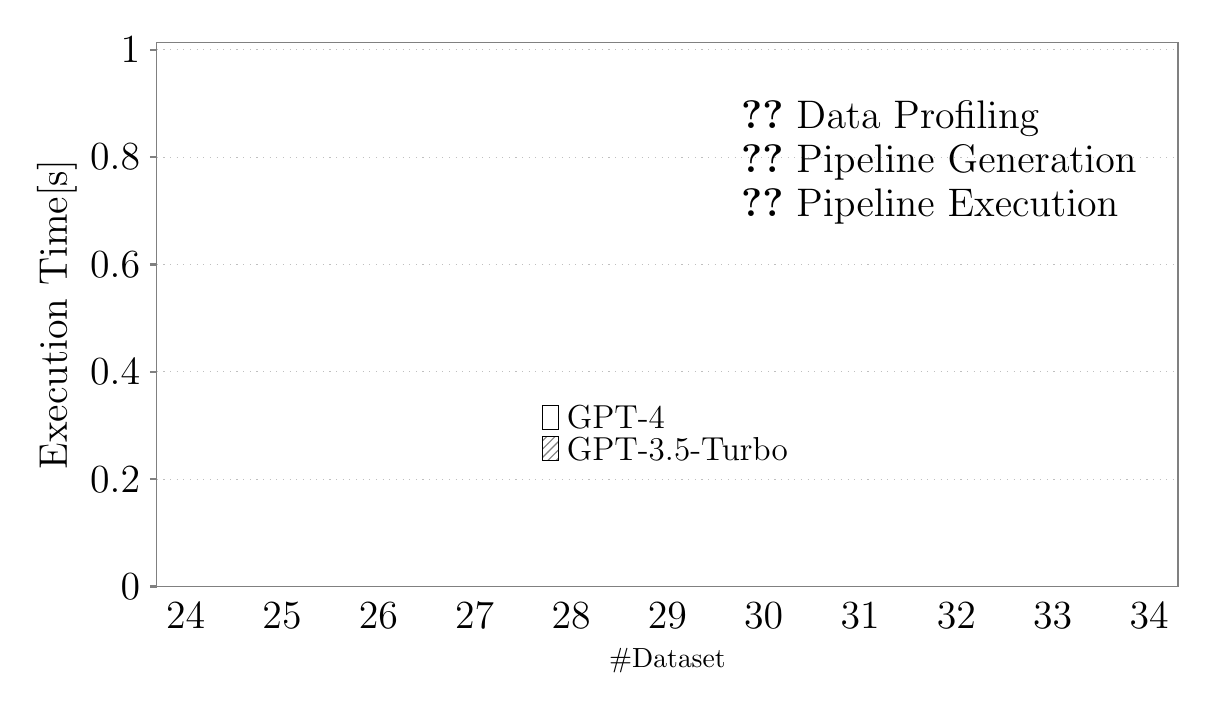
\begin{tikzpicture}[
  %ymode=log,  
  every axis/.style={
    ybar stacked,
    %ymode=log,
    xtick style={draw=none},		
    every major tick/.append style={ thick,major tick length=2.5pt, gray},
    axis line style={gray},
    ybar,        
    ybar=0pt,
    ymin=0,
    ymax=1400,
    log ticks with fixed point,
    y tick label style={/pgf/number format/1000 sep={}},
    x tick label style={/pgf/number format/1000 sep={}},
    scaled y ticks=false,
    enlarge y limits={0.013,upper},
    enlarge x limits=0.03,
    ylabel={Execution Time[s]},
    xlabel={$\#$Dataset},
    ytick={0,200,400,600,800,1000,1200,1400},
    %yticklabels={0,10,100,1e3,1e4},
    ytick align=outside,
    xtick pos=left,
    ytick pos=left,
    yticklabel style = {font=\Large},
    ylabel style = {font=\Large, yshift=-2pt},
    xticklabel style = {font=\Large, xshift=0pt},
    xtick=data,
    height=0.7\columnwidth,
    width=1.2\columnwidth,    
    bar width=6pt,	 
    ymajorgrids=true,
    grid style=dotted,   
    minor grid style={gray!50},  
    symbolic x coords={covertype,dionis,connect-4,Fashion-MNIST,helena,jannis,jungle_chess_2pcs_raw_endgame_complete,robert,shuttle,volkert,car,cnae-9,dilbert,fabert,mfeat-factors,segment,vehicle,airlines,albert,adult,Amazon_employee_access,APSFailure,bank-marketing,guillermo,higgs,KDDCup09_appetency,MiniBooNE,nomao,numerai28.6,riccardo,Australian,blood-transfusion-service-center,christine,credit-g,jasmine,kc1,kr-vs-kp,phoneme,sylvine},   
    xticklabels={23,24,25,26,27,28,29,30,31,32,33,34,35,36,37,38,39},    
    legend image code/.code={\draw [#1] (0cm,-0.1cm) rectangle (0.2cm,0.3cm); },
  }	 
]
	
\begin{axis}  
	\addplotCatDB{gpt-3.5-turbo}{12pt}{6pt}{0pt}{pattern=north east lines,pattern color=gray};
\end{axis}

\begin{axis}[hide axis] %
    \addplotCatDB{gpt-4}{6}{0pt}{-6pt}{};	  	  
\end{axis}	



\node [draw=none,inner sep=0, font=\Large, anchor=west] (leg1) at (rel axis cs: 0.6,0.78) {\shortstack[l]{
			\ref{legprofile} Data Profiling \\
      \ref{legcode} Pipeline Generation  \\
			\ref{legpipeline} Pipeline  Execution 			 			
	}};
\draw[draw=black] (4.9,2) rectangle (5.1cm,2.3cm); 
\node [draw=none,inner sep=0, font=\large, anchor=west] (gpt-4) at (5.2,2.15) {GPT-4};

\draw[pattern=north east lines, pattern color=gray] (4.9,1.6) rectangle (5.1cm,1.9cm);
\node [draw=none,inner sep=0, font=\large, anchor=west] (gpt-4) at (5.2,1.75) {GPT-3.5-Turbo};

\end{tikzpicture}

    %     \caption{Runtime}
    % \end{figure*}  

    % \tikzsetnextfilename{Experiment1-CatDB-Runtime-Regression}
    % \begin{figure*}[h]
    %     \centering
    %     \newcommand{\addplotCatDB}[6]{
	   \addplot[xshift=#1,draw=black,line width=0.15pt, fill=tugb, discard if singlecatdb={#2}{#3}{#4},postaction={#5}] 
	   table[ y=llm_pipe_gen_time, col sep=comma, x=dataset] {results/Experiment_CatDB_Micro_Benchmark.dat};
	   \label{leg_pip_gen_#4}

     \addplot[xshift=#6,draw=black,line width=0.15pt, fill=tug, discard if singlecatdb={#2}{#3}{#4},postaction={#5}] 
	   table[ y=llm_pipe_run_time, col sep=comma, x=dataset] {results/Experiment_CatDB_Micro_Benchmark.dat};
	   \label{leg_pip_runtime_#4}       
};

\newcommand{\addplotDataProfilling}[2]{
	   \addplot[xshift=#1, draw=black,line width=0.15pt, fill=black, discard if singlecatdb={gpt-4}{#2}{SCHEMA}] 
	   table[ y=data_profile_time, col sep=comma, x=dataset] {results/Experiment_CatDB_Micro_Benchmark.dat};
     \label{leg_dataprofile} 
};


\pgfplotsset{
    discard if singlecatdb/.style n args={3}{
        x filter/.code={
            \edef\tempa{\thisrow{llm_model}}
            \edef\tempb{#1}
            \ifx\tempa\tempb
                    \edef\tempc{\thisrow{task_type}}
                    \edef\tempd{#2}
                    \ifx\tempc\tempd
                      \edef\tempe{\thisrow{prompt_representation_type}}
                      \edef\tempf{#3}
                      \ifx\tempe\tempf                        	
                      \else
                      \def\pgfmathresult{inf}
                      \fi
                    \else
                    \def\pgfmathresult{inf}
                    \fi      
            \else
            \def\pgfmathresult{inf}
            \fi			
        }
    },
    discard if profile/.style n args={1}{
      x filter/.code={
          \edef\tempa{\thisrow{task_type}}
          \edef\tempb{#1}
          \ifx\tempa\tempb
          \else
          \def\pgfmathresult{inf}
          \fi			
      }
  },
};

\begin{tikzpicture}[
  %ymode=log,  
  every axis/.style={
    major x tick style = {draw=none},
    ybar stacked,
    %ymode=log,
    xtick style={draw=none},		
    every major tick/.append style={ thick,major tick length=2.5pt, gray},
    axis line style={gray},
    ybar,        
    ybar=0pt,
    ymin=0,
    ymax=260,
    log ticks with fixed point,
    y tick label style={/pgf/number format/1000 sep={}},
    x tick label style={/pgf/number format/1000 sep={}},
    scaled y ticks=false,
    enlarge y limits={0.013,upper},
    enlarge x limits=0.1,
    ylabel={Execution Time[s]},
    %xlabel={$\#$Dataset},
    ytick={0,50,100, 150,200,250},
    %yticklabels={0,1e2, 1e3,1e4},
    ytick align=outside,
    xtick pos=left,
    ytick pos=left,
    yticklabel style = {font=\Large},
    ylabel style = {font=\Large, yshift=-2pt},
    xticklabel style = {font=\normalsize, xshift=0pt},
    height=0.7\columnwidth,
    width=1.45\columnwidth,    
    bar width=8pt,	 
    ymajorgrids=true,
    grid style=dotted,   
    minor grid style={gray!50}, 
    xtick = data,
    symbolic x coords={Microsoft,CMC,Diabetes,Pokerhand,Sudoku Puzzles,Higgs,Simulated Electricity,Credit g,Airlines,KDD98,Zurich Transport,Federal Election,Black Friday,Buzzinsocialmedia,NYC}, 
    %xtickmin=simulated_electricity,
    %xtickmax=federal_election,
    %xticklabels={Simulated Electricity,Higgs,KDD98,Airlines,Credit g},   
    legend image code/.code={\draw [#1] (0cm,-0.1cm) rectangle (0.3cm,0.2cm); },
  }	 
]
	
\begin{axis}%[hide axis]
  \addplotDataProfilling{-16pt}{regression};	  	  
\end{axis}

\begin{axis}[hide axis]  
  \addplotCatDB{-4}{gpt-4}{regression}{SCHEMA}{}{-12};
\end{axis}

\begin{axis}[hide axis]  
	\addplotCatDB{4}{gpt-4}{regression}{SCHEMA_STATISTIC}{pattern=north east lines,pattern color=gray!130}{-4};
\end{axis}

	
\node [draw=none,inner sep=0, font=\Large, anchor=west] (leg1) at (rel axis cs: 0.15,0.80) {\shortstack[l]{
			\ref{leg_dataprofile} Data Profiling \\
      \ref{leg_pip_gen_SCHEMA} Pipeline Generation  \\
			\ref{leg_pip_runtime_SCHEMA} Pipeline Execution 			 			
	}};

 \node [draw=none,inner sep=0, font=\large, anchor=west, below=of leg1, yshift=20pt, xshift=-22pt] (schema) {Schema};
 \draw[draw=black] ($(schema.west)+(-0.4cm,.15cm)$) rectangle ($(schema.west)+(-0.1cm,-0.15cm)$); 


 \node [draw=none,inner sep=0, font=\large, anchor=west, right=of schema,yshift=0pt] (schema_statistic)  {Schema \& Statistics};
 \draw[draw=black, pattern=north east lines, pattern color=gray!130] ($(schema_statistic.west)+(-0.4cm,.15cm)$) rectangle ($(schema_statistic.west)+(-0.1cm,-0.15cm)$); 

\end{tikzpicture}

    %     \caption{Runtime}
    % \end{figure*}  

\end{document}
\endinput
